\documentclass[a4paper]{article}

\usepackage{url,afterpage,amssymb,amsfonts}
\usepackage{enumitem,makecell}
\usepackage{booktabs}
%\usepackage{times}
%\usepackage{amsthm}
%\usepackage[ruled,linesnumbered]{algorithm2e}
\usepackage{multirow}
\usepackage{array}
\usepackage{subfig}
\usepackage{graphicx}
\usepackage{amsmath}
\usepackage{verbatim}
%\usepackage{algorithmic}
\usepackage{algpseudocode}

\usepackage{color}
\usepackage{colortbl}
% \usepackage{tikz}
% \usetikzlibrary{decorations.pathmorphing}
\graphicspath{{./figs/}}
%\usepackage[ruled,vlined]{algorithm2e}
%\usepackage{algorithm}% http://ctan.org/pkg/algorithm
\usepackage[linesnumbered,ruled]{algorithm2e}% http://ctan.org/pkg/algorithm
\usepackage{hyperref}

\usepackage{xcolor}
\usepackage{listings}
\usepackage{soul}
%\usepackage{natbib}
%\usepackage[square,sort,comma,numbers]{natbib}
\usepackage{subfig}
\usepackage{url,afterpage,amssymb,amsfonts}
\usepackage{enumitem,makecell}
\usepackage{color}
\usepackage{colortbl}
\usepackage{float}
\usepackage{wrapfig}
\usepackage{inputenc}
\usepackage{tabularx}
\usepackage{pgfgantt}
\usepackage{graphicx}
\usepackage[export]{adjustbox}
\usepackage{xcolor}
\usepackage{tikz}
\usetikzlibrary{shapes.geometric, arrows}

%\usepackage[font=footnotesize]{caption}
\date{\vspace{-5ex}}

\setlength{\topmargin}{-10mm}
%\setlength{\textwidth}{7in}
%\setlength{\oddsidemargin}{-5mm}
%\setlength{\textheight}{9in}
%\setlength{\footskip}{1in}

\usepackage{geometry}
\geometry{
	a4paper,
	total={170mm,257mm},
	left=25mm,
	right=25mm,
	top=25mm,
	bottom=25mm
}

\newcommand\todo[1]{\textcolor{red}{#1}}

\begin{document}

\fontsize{11}{15}
\selectfont
\begin{titlepage}
	\begin{center}
		\vspace*{1cm}
		
		\Huge
		\textbf{Project on Unsupervised Text to Gloss Translation}	
		
		
		\vspace{0.3cm}
		\LARGE
		 (Deep Learning for Low Resource NLP)
		\vspace{1.3cm}
		
		%\textbf{Research Initiation Grant}
		
		\vspace{2.3cm}
  
		\textbf{Umesh Kashyap} \\
		\vspace{0.2cm}
		{Roll No. - 12210830} \\
            \href{mailto:xxx@iitbhilai.ac.in}{umeshk@iitbhilai.ac.in} \\
	
		
		\textbf{Gowry Sailaja V} \\
		\vspace{0.2cm}
		{Roll No. - 42200090} \\
            \href{mailto:xxx@iitbhilai.ac.in}{sailajav@iitbhilai.ac.in} \\
		
		\vspace{0.2cm}
            \textbf{Kartikeya Saraswat} \\
		\vspace{0.2cm}
		{Roll No. - 12110080} \\
            \href{mailto:xxx@iitbhilai.ac.in}{kartikeyas@iitbhilai.ac.in} \\
		
		\vspace{0.2cm}
  
		\vspace{0.2cm}
		
		\vspace{2.4cm}	
            Group Ph.D \\ 
		Department of CSE - DSAI \\
		\vspace{0.2cm}
		Indian Institute of Technology Bhilai \\
		
		\vspace{0.2cm} 		
		\today
		
	\end{center}
\end{titlepage}

\tableofcontents
\clearpage

\pagenumbering{arabic}


\newpage
\section{Abstract} \label{sec:abstract}

Unsupervised mode is important in the current setup as it allows for pre-training on large amounts of unpaired data, such as monolingual data, which is more easily accessible compared to paired data. This helps in addressing the low-resource scenario and enables the transfer of knowledge from the pre-training task to downstream language generation tasks. Pre-training in an unsupervised manner allows the model to learn general language patterns and representations, which can then be fine-tuned on specific downstream tasks. This fine-tuning process further improves the performance by adapting the pre-trained model to the target task, leveraging the limited available paired or unpaired data.

Unsupervised masked sequence to sequence pre-training, such as MASS \cite{ref_paper}, is important for language generation tasks as it allows for the transfer of knowledge from a rich-resource pre-training task to low/zero-resource downstream tasks. MASS adopts the encoder-decoder framework to reconstruct a sentence fragment given the remaining part of the sentence, which helps in developing the capability of representation extraction and language modeling. The effectiveness of the design choices in MASS, such as masking consecutive tokens in the encoder side and masking input tokens of the decoder that are not masked in the encoder side, helps in building better language modeling capability and encouraging the decoder to extract more useful information from the encoder side. 

In our work, we have used the MASS model on German text to Gloss which is low resource in terms of dataset size as the availability of parallel data is limited. Through the work, we tried to produce a quality gloss through the model referred.  




\section{Introduction} \label{sec:Introduction}

\subsection{Background}
The goal of sign language translation, or SLT, is to eliminate communication barriers between the hearing and the deaf or hard-of-hearing communities. The fact that Sign Languages (SLs) are multi-channeled, non-written languages presents a challenge for SLT. As such, the recent advances in text-based machine translation (MT) cannot be easily applied to machine translation (MT) for SLs. Glosses are one of these representations, in which words from the appropriate spoken language—often with affixes and markers—are used to name signals. Glosses enable the system to be built in two stages: text-to-gloss translation and generation of videos. In our work, we are focusing on generation of quality gloss using unsupervised language generation task.


\subsection{Contributions}
\begin{enumerate}
\item Quality gloss generation using unsupervised masked sequence to sequence pre-training in the context of unavailability of parallel data.
\item Fine-tuning on unsupervised NMT using monolingual data for training and back-translation to generate pseudo bilingual data.
\end{enumerate}
\section{Problem Statement} \label{sec:problem statement}
The task of language production, particularly in low-resource circumstances where there is little or no paired data available for training, is the problem that our study attempts to solve. In our work, we are using an encoder-decoder framework to put a sentence fragment back together given the parts that are left. The aim is to train the encoder and decoder to enhance their ability to extract representations and model languages.
\section{Literature Survey or Earlier works} \label{sec: literature survey}

 The work \cite{DBLP} introduces BERT, a pre-training method for language understanding tasks. BERT utilizes a masked language modeling objective and next sentence prediction to learn contextualized word representations. It achieved state-of-the-art results on various language understanding benchmarks. The paper \cite{gen_pretrain} presents a generative pre-training approach called OpenAI GPT. It uses a transformer-based architecture and trains a language model on a large corpus of unlabeled text. OpenAI GPT achieves impressive performance on language understanding tasks and demonstrates the effectiveness of generative pre-training. The paper \cite{attention} introduces the Transformer model, which relies solely on self-attention mechanisms for sequence transduction tasks. The Transformer model achieves state-of-the-art results on machine translation tasks and eliminates the need for recurrent or convolutional layers. Neural Machine Translation by Jointly Learning to Align and Translate \cite{nmt} proposes an attention-based neural machine translation (NMT) model. It introduces the concept of attention mechanisms to align and translate source and target sentences. The attention-based NMT model significantly improves translation quality compared to traditional NMT models. Deep Contextualized Word Representations \cite{word_reps} presents a deep contextualized word representation model. ELMo generates word embeddings that capture both word-level and context-sensitive features. It achieves state-of-the-art results on various language understanding tasks, demonstrating the effectiveness of contextualized word representations. Sequence to Sequence Learning with Neural Networks \cite{seq_to_seq} introduces the sequence-to-sequence learning framework for neural networks. It demonstrates the effectiveness of using encoder-decoder architectures for various language generation tasks, including machine translation, text summarization, and conversational response generation. Massive Exploration of Neural Machine Translation Architectures \cite{massive_nmt} explores various neural machine translation (NMT) architectures and their impact on translation quality. It investigates different encoder and decoder architectures, attention mechanisms, and training techniques. The study provides insights into the design choices for NMT models and their effects on translation performance. "Neural Machine Translation Methods for Translating Text to Sign Language Glosses" \cite{base_paper} explores state-of-the-art techniques for improving machine translation of spoken language text to sign language glosses. The authors propose methods such as data augmentation, semi-supervised NMT, transfer learning, and multilingual NMT. They experiment with two German sign language corpora and achieve significant improvements in translation performance, outperforming previous work on the same test set. The best setting combines multilingual NMT with data augmentation and is also validated on an American Sign Language corpus. Data augmentation is a common technique used to address low resource conditions in machine translation. It involves adding synthetically generated data from various sources to the training dataset. This technique aims to increase the size and diversity of the data, making the model more robust and capable of handling variable appearances of the spoken language sentences. In the context of sign language gloss translation, data augmentation \cite{data_augmenta} has been explored to improve translation performance. 
\section{Novelty} \label{sec: Novelty}
The work \cite{base_paper} focused on the gloss generation using semi-supervised neural machine translation system. In our work, we attempted to generate the quality gloss using unsupervised neural machine translation \cite{nmt}. 
\section{Experiments} \label{sec: experiments}



\subsection{Experiment 1}
 Eliminating the need of cross-lingual information and we attempted to train NMT systems in a completely unsupervised manner, relying solely on monolingual corpora.


\subsubsection{Experimental architecture}
Architecture of the proposed system \ref{unsupervised_NMT}. For each sentence in language L1, the system is trained alternating two steps: denoising, which optimizes the probability of encoding a noised version of the sentence with the shared encoder and reconstructing it with the L1 decoder, and on-the-fly backtranslation, which translates the sentence in inference mode (encoding it with the shared encoder and decoding it with the L2 decoder) and then optimizes the probability of encoding this translated sentence with the shared encoder and recovering the original sentence with the L1 decoder. Training alternates between sentences in L1 and L2, with analogous steps for the latter.

 \begin{figure} [h]
    \center
    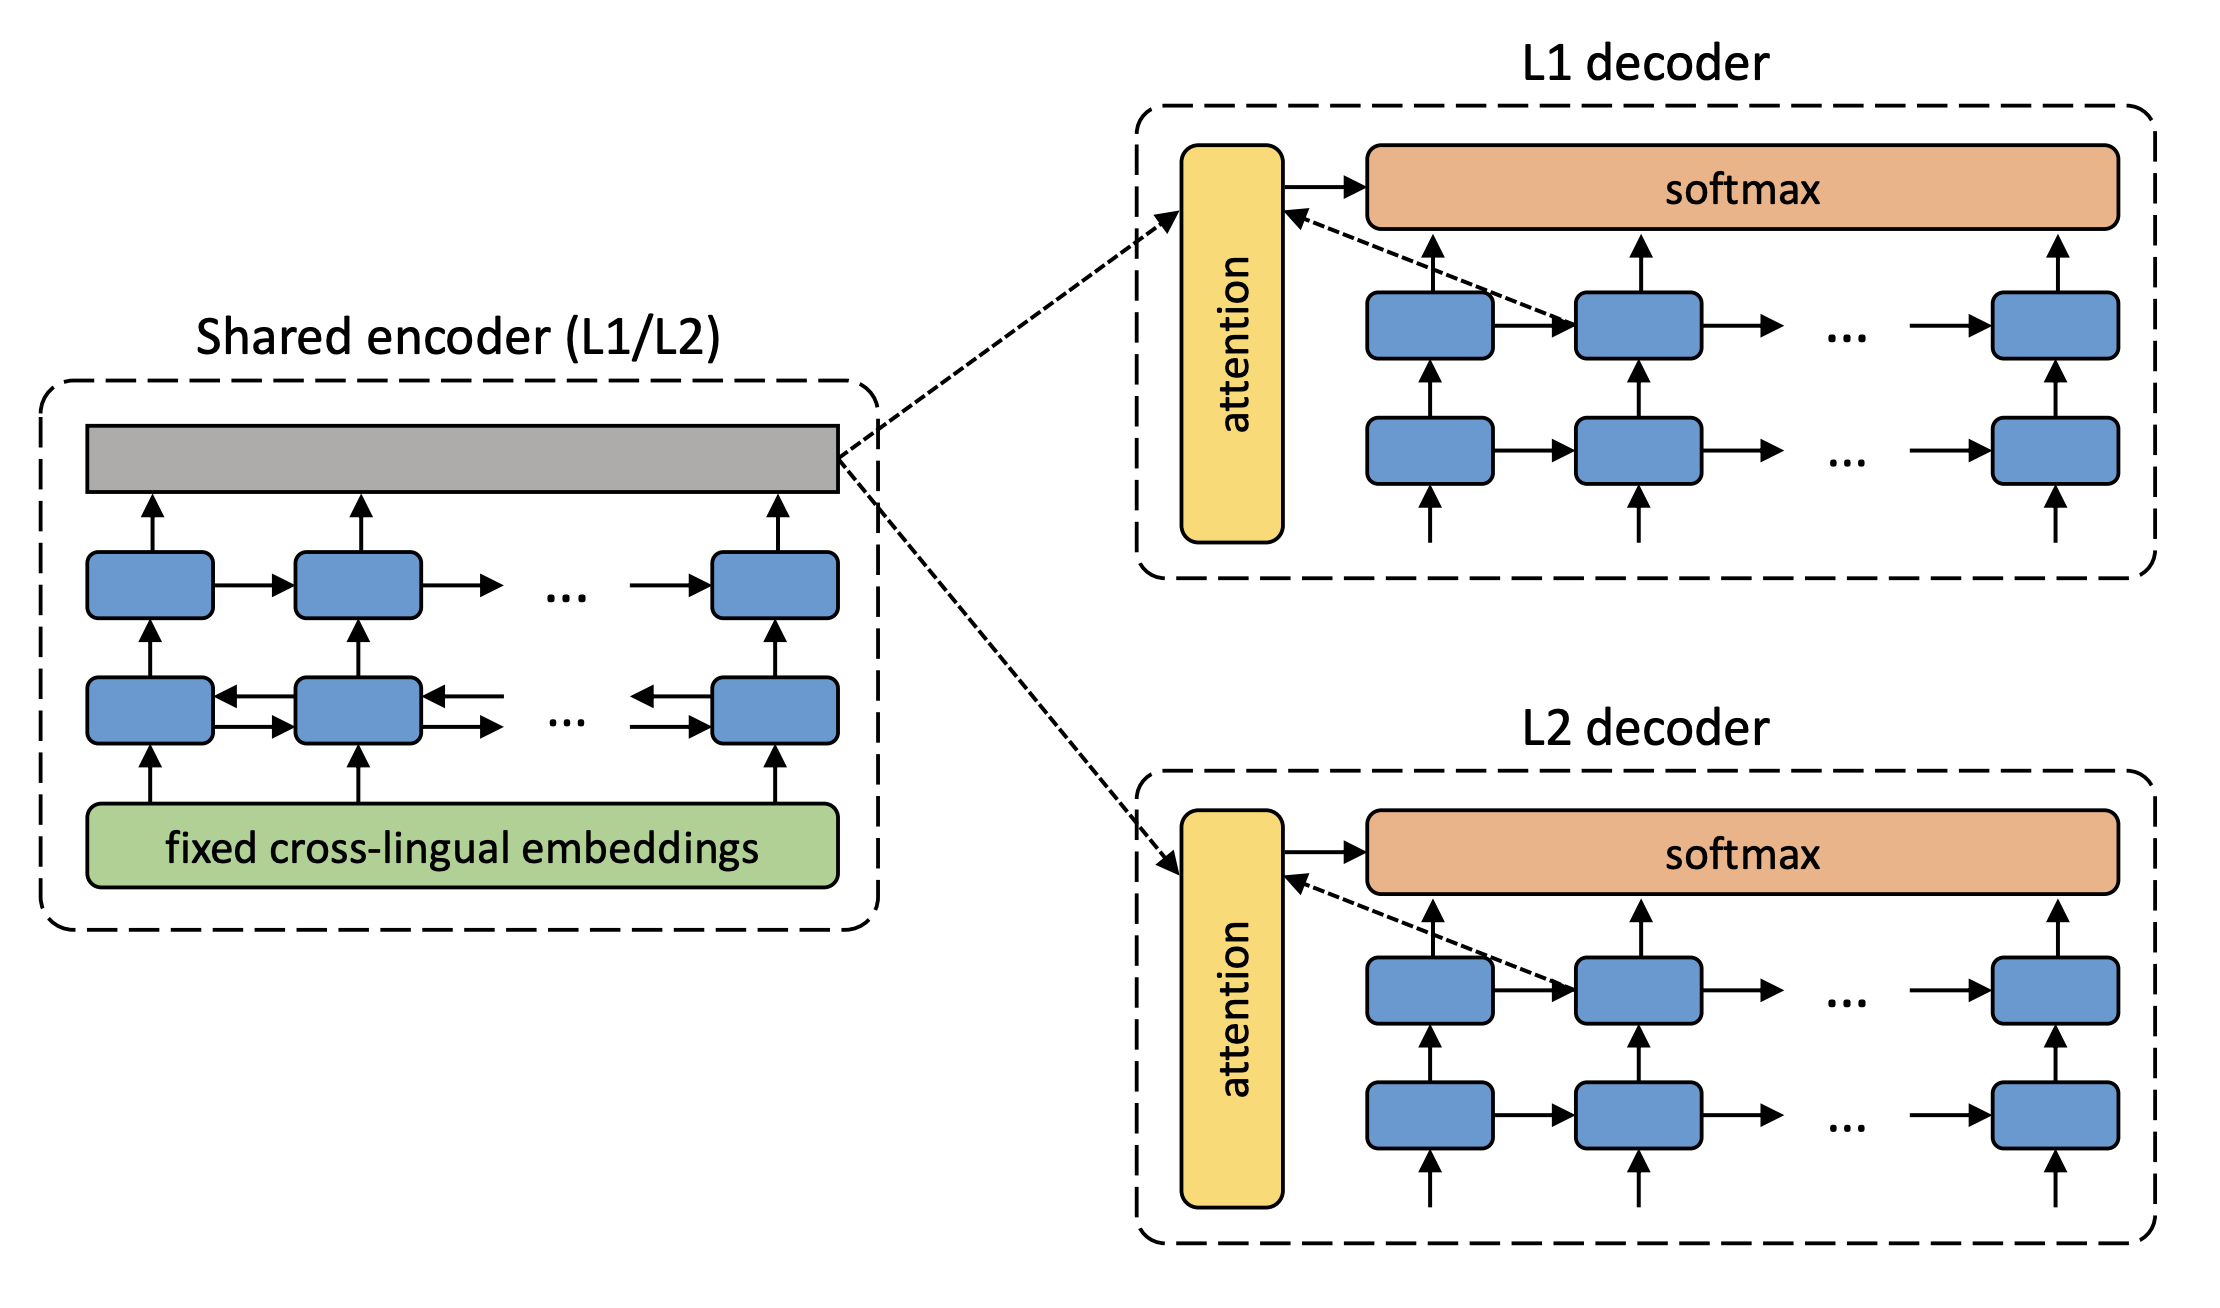
\includegraphics[width=8cm]{Figures/unsup_nmt.png}  
    \caption{Proposed System}
    \label{unsupervised_NMT}
\end{figure}

\subsubsection{Experimental settings}
\begin{enumerate}
    \item Unsupervised: This is the main scenario under consideration in our work, where the system has access to nothing but monolingual corpora.
    \item The systems are evaluated using tokenized BLEU scores as computed by the multi-bleu.perl script. 
    \item For the corpus preprocessing, tokenization and true casing using standard Moses are performed.
    \item Learning was done on the monolingual corpus of each language independently. 
    \item Experiments at the word level in this unsupervised scenario, limiting the vocabulary to the most frequent tokens and replacing the rest with a special token $<$UNK$>$. 
    \item Used the monolingual corpora to independently train the embeddings for each language using word2vec.
    \item we use the skip-gram model with ten negative samples, a context window of ten words, 300 dimensions, a sub-sampling of $10^{-5}$, and ten training iterations.
    \item The training of the proposed system itself is done using the procedure described with the cross-entropy loss function and a batch size of 50 sentences.
    

\end{enumerate}


\subsection{Experiment 2}
Experimental details about MASS pre-training and fine-tuning on a variety of language generation tasks are given as follows:


\subsubsection{Experimental architecture}

 \begin{figure} [h]
    \center
    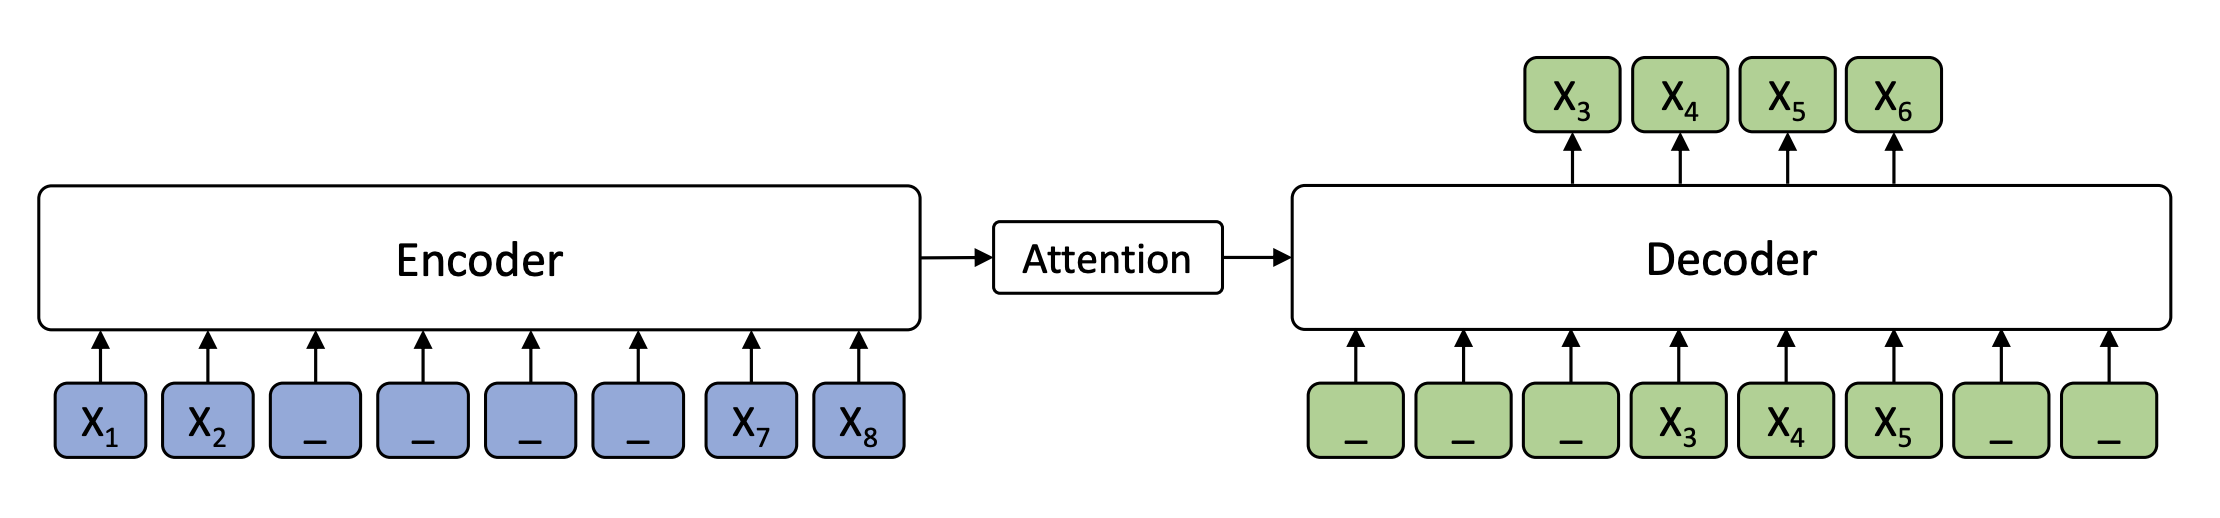
\includegraphics[width=8cm]{Figures/mass.png}  
    \caption{The Encoder-Decoder Framework}
    \label{en_dec_framework}
\end{figure}


\subsubsection{Experimental settings}
\begin{enumerate}
    \item Model Configuration : 
    Transformer as the basic model structure, which consists of 6-layer encoder and 6-layer decoder with 1024 embedding/hidden size and 4096 feed-forward filter size. 
    \item Pre-train the model on the monolingual data of the source and target languages.
    \item To distinguish between the source and target languages in neural machine translation task, a language embedding is added to each token of the input sentence for the encoder and decoder, which is also learnt end-to-end. 
    \item Dataset : 
\end{enumerate}
\section{Results and Analysis} \label{sec: baselines}

\subsection{Results of Experiment 1}
BLEU score on testing data : 0.0078

\subsection{Results of Experiment 2}
BLEU score on testing data : 0.077

\bibliographystyle{plain}
\newpage
\bibliography{references/references}
\end{document}




